% --------------------------------------------------------------
% This is all preamble stuff that you don't have to worry about.
% Head down to where it says "Start here"
% --------------------------------------------------------------

\documentclass[12pt]{article}
\usepackage[margin=0.75in]{geometry}
\usepackage{amsmath,amsthm,amssymb,mathtools,graphicx,enumitem,hyperref,hyphenat,float}
% \usepackage[paperwidth=\maxdimen,paperheight=\maxdimen]{geometry}
\usepackage{svg}
\usepackage{register}
\usepackage{rotating}
\DeclarePairedDelimiter{\ceil}{\lceil}{\rceil}
\newcommand{\N}{\mathbb{N}}
\newcommand{\Z}{\mathbb{Z}}
\newcommand{\Q}{\mathbb{Q}}
\newcommand{\R}{\mathbb{R}}
\newcommand{\F}{\mathbb{F}}
\newcommand{\C}{\mathbb{C}}
\newcommand{\lub}{\mathrm{lub}}
\newcommand{\g}{\mathrm{glb}}
\newcommand{\seq}{\subseteq}
\newcommand{\e}{\epsilon} 
\newcommand{\de}{\delta}
\newcommand{\mbf}{\mathbf}
\newcommand{\es}{\emptyset}
\newcommand{\mc}{\mathcal}
\newcommand{\un}{\cup}
\newcommand{\ic}{\cap}
\newcommand{\gen}[1]{\ensuremath{\langle #1\rangle}}
\newcommand{\spn}{\mathrm{span \ }}
\newcommand{\dm}{\mathrm{dim \ }}
\newcommand{\Lm}{\mathcal{L}}
\newcommand{\nll}{\mathrm{null \ }}
\newcommand{\rng}{\mathrm{range \ }}
\newcommand{\dgr}{\mathrm{deg \ }}
\newcommand{\Lim}{\lim\limits}
\newcommand{\Sum}{\sum\limits}
\newcommand{\Pt}{\|P\|}
\newcommand{\dmn}{\mathrm{dom \ }}
\newcommand{\Prod}{\prod\limits}
\DeclarePairedDelimiter\floor{\lfloor}{\rfloor}
\DeclarePairedDelimiter\ev{\langle}{\rangle}
\newcommand*\dif{\mathop{}\!\mathrm{d}}
\newcommand{\Beta}{\mathcal B}
\newcommand{\Seq}{\mathrm{Seq }}
\theoremstyle{plain}

\newtheorem{thm}{Theorem} % reset theorem numbering for each chapter
\newtheorem{lem}{Lemma}
\newtheorem{cor}{Corollary}
\newtheorem{rem}{Remark}
\newtheorem{fct}{Fact}
\newtheorem{cnj}{Conjecture}
\newtheorem{asm}{Assumption}
\theoremstyle{definition}
\newtheorem{defn}{Definition}
\newtheorem{exmp}{Example} % same for example numbers
\renewcommand{\regBitWidth}{16}
	
\begin{document}
	
% --------------------------------------------------------------
%                         Start here
% --------------------------------------------------------------
	
\begin{titlepage}

	\newcommand{\HRule}{\rule{\linewidth}{0.5mm}} % Defines a new command for the horizontal lines, change thickness here
	
	\center % Center everything on the page
	 
	%----------------------------------------------------------------------------------------
	%	HEADING SECTIONS
	%----------------------------------------------------------------------------------------
	
	\textsc{\LARGE Faculty of Engineering, Cairo University}\\[0.5cm] % Name of your university/college
	\textsc{\large Computer Engineering Department}\\[1.5cm] % Minor heading such as course title
	
	\textsc{\Large Computer Architecture Course Project}\\[0.5cm] % Major heading such as course name
	
	%----------------------------------------------------------------------------------------
	%	TITLE SECTION
	%----------------------------------------------------------------------------------------
	
	\HRule \\[0.4cm]
	{ \huge \bfseries Orthrus - Phase 1 Report}\\[0.4cm] % Title of your doc
	\HRule \\[1.5cm]
	 
	%----------------------------------------------------------------------------------------
	%	AUTHOR SECTION
	%----------------------------------------------------------------------------------------
	
	\begin{minipage}{0.4\textwidth}
	\begin{flushleft} \large
	Ahmad Khaled \\
	Maryam Shalaby \\
	Zeinab Rabie \\
	Omnia Zakaria
	\end{flushleft}
	\end{minipage}
	\begin{minipage}{0.4\textwidth}
	\begin{flushright}\large
        Section 1 BN. 03 \\
        Section 2 BN. 21 \\
        Section 1 BN. 22 \\
        Section 1 BN. 23 \\
	\end{flushright}
	\end{minipage}\\[1cm]
	
	% If you don't want a supervisor, uncomment the two lines below and remove the section above
	%\Large \emph{Author:}\\
	%John \textsc{Smith}\\[3cm] % Your name
	
	%----------------------------------------------------------------------------------------
	%	LOGO SECTION
	%----------------------------------------------------------------------------------------
	
	
\includegraphics[scale=0.15]{cu_logo.png}\\[1cm] % Include a department/university logo - this will require the graphicx package
	 
	%----------------------------------------------------------------------------------------
	
	\vfill % Fill the rest of the page with whitespace
	
\end{titlepage}

\tableofcontents

\section{Introduction}
Orthrus is a pipelined static dual-issue microprocessor implementing a RISC ISA similar to the MIPS ISA. In the following sections we outline the instruction format, the general design of the processor, as well as the pipeline stages design.

\section{Instruction Set Architecture}
    The structure for the IR for One-Operand instructions is given in Figure~\ref{IR-1op}.The structure for the IR for Two-Operand instructions is given in Figure~\ref{IR-2op}. The structure for the IR for Memory instructions is given in Figure~\ref{IR-memory}. The structure for the IR for Branch $\&$ Change of Control instructions is given in Figure~\ref{IR-Branch}.
    \begin{table}[H]
        \centering
        \begin{tabular}{c|c|c|c|c|}
            \cline{2-5}
                            & $R_0$ & $R_1$ & $R_2$ & $R_3$ \\ \cline{2-5} 
            \textit{Code}   & 000      & 001            & 010            & 011     \\ \cline{2-5} 
                            & $R_4$ & $R_5$ & $R_6?$ & $R_7$ \\ \cline{2-5} 
            \textit{Code}   & 100      & 101            & 110            & 111     \\ \cline{2-5} 
        \end{tabular}
        \caption{Register Addressing Codes}
        \label{reg-addr-codes}
    \end{table}
    \begin{table}[H]
        \centering
        \begin{tabular}{|c|c|c|c|c|c|c|c|c|}
            \hline
            Instruction  & NOP & SETC & CLRC  & NOT & INC & DEC & OUT & IN  \\ \hline
            OP Code     & 00000 & 00001 & 00010 & 00011 & 00100 & 00101 & 00110 & 00111 \\ \hline
        \end{tabular}
        \caption{One-Operand Instruction Codes}
        \label{One_Op Opcodes}
    \end{table}
    
    \begin{figure}[H]
        \centering
        \caption{IR Structure For One-Operand Instructions}
        \label{IR-1op}
        \vspace{0.5 cm}
        \regfield{}{5}{11}{{Instruction}}
        \regfield{}{3}{8}{{Destination Register}}
        \regfield{}{8}{0}{{}}
        \\
        \vspace{0.5 cm}
        \begin{regdesc}\begin{reglist}
            \item [Instruction] specifies the instruction to execute. Possible codes given in. Table~\ref{One_Op Opcodes}.
            \item [Destination Register] specifies the destination register. Possible codes given in Table~\ref{reg-addr-codes}.
        \end{reglist}\end{regdesc}
    \end{figure}
    
    \begin{table}[H]
        \centering
        \begin{tabular}{|c|c|c|c|c|c|c|c|}
            \hline
            Instruction & MOV & ADD & SUB & AND & OR & SHL & SHR \\ \hline
            OP Code     & 01000 & 01001 & 01010 & 01011 & 01100 & 01101 & 01110  \\ \hline
        \end{tabular}
        \caption{Two-Operand Instruction Codes}
        \label{Two_Op Opcodes}
    \end{table}
    
    \begin{figure}[H]
        \centering
        \caption{IR Structure For Two-Operand Instructions}
        \label{IR-2op}
        \vspace{0.5 cm}
        \regfield{}{5}{11}{{Instruction}}
        \regfield{}{3}{8}{{Source Register}}
        \regfield{}{3}{5}{{Destination Register}}
        \regfield{}{4}{1}{{Shift Amount}}
        \regfield{}{1}{0}{{}}
        \\
        \vspace{0.5 cm}
        \begin{regdesc}\begin{reglist}
            \item [Instruction] specifies the instruction to execute. Possible codes given in. Table~\ref{Two_Op Opcodes}.
            \item [Source Register] specifies the source register. Possible codes given in Table~\ref{reg-addr-codes}.
            \item [Destination Register] specifies the destination register. Possible codes given in Table~\ref{reg-addr-codes}.
            \item [Shift Amount] specifies the number of bits to shift the source Register by.
        \end{reglist}\end{regdesc}
    \end{figure}
    \begin{table}[H]
        \centering
        \begin{tabular}{|c|c|c|c|c|c|}
            \hline
            Instruction & PUSH  & POP  & LDM  & LDD  & STD   \\ \hline
            OP Code     & 01111 & 10000 & 10001 & 10010 & 10011 \\ \hline
        \end{tabular}
        \caption{Memory Instruction Codes}
        \label{memory opCodes}
    \end{table}
    \begin{figure}[H]
        \centering
        \caption{IR Structure For Memory Instructions}
        \label{IR-memory}
        \vspace{0.5 cm}
        \regfield{}{5}{11}{{Instruction}}
        \regfield{}{3}{8}{{Source Register}}
        \regfield{}{3}{5}{{Destination Register}}
        \regfield{}{5}{0}{{}} \\
        \vspace{0.5 cm}
        \begin{regdesc}\begin{reglist}            
            \item [Instruction] specifies the instruction to execute. Possible codes given in Table~\ref{memory opCodes}.
            \item [Source Register] specifies the Source Register. Possible codes given in Table~\ref{reg-addr-codes}.
            \item [Destination Register] specifies the Destination Register. Possible codes given in Table~\ref{reg-addr-codes}.
        \end{reglist}\end{regdesc}
    \end{figure}
    \begin{table}[H]
        \centering
        \begin{tabular}{|c|c|c|c|c|c|c|c|}
            \hline
            Instruction & JZ  & JN & JC  & JMP  & CALL  & RET  & RTI \\ \hline
            OP Code     & 10100 & 10101 & 10110 & 10111 & 11000 & 11001 & 11010 \\ \hline
        \end{tabular}
        \caption{Branch $\&$ Change of Control Instruction Codes}
        \label{Branch Opcodes}
    \end{table}
    \begin{figure}[H]
        \centering
        \caption{IR Structure For Branch $\&$ Change of Control Instruction}
        \label{IR-Branch}
        \vspace{0.5 cm}
        \regfield{}{5}{11}{{Instruction}}
        \regfield{}{3}{8}{{Destination Register}}
        \regfield{}{8}{0}{{}} \\
        \vspace{0.5 cm}
        \begin{regdesc}\begin{reglist}            
            \item [Instruction] specifies the instruction to execute. Possible codes given in Table~\ref{Branch Opcodes}.
            \item [Destination Register] specifies the destination register. Possible codes given in Table~\ref{reg-addr-codes}.
        \end{reglist}\end{regdesc}
    \end{figure}
\pagebreak

\section{Design}
\subsection{Overall System Schematic}
Figure~\ref{sys-schematic-1} and Figure~\ref{sys-schematic-2} show the overall design of Orthrus, along with the main connections. Note that some of the connections specific to hazards and forwarding are omitted for clarity, and that some of the connections between pipeline register buffers are also omitted for clarity (but if two registers share the same name across two register buffers then they should be connected). The units in each stage are responsible for generating control signals for themselves given the inputs from the previous stage, from the memory, and from the Hazard/Forwarding unit. In the following subsections, we discuss each unit shown in the diagram in detail. We mostly suppress the details of hazard handling by assuming that all the units mentioned always have a \textbf{stall} input and a \textbf{flush} input that cause the unit to stall its corresponding stage (by propagating a No-Op to the next instruction) or flush whatever instruction is in it (by propagating a No-Op to the next instruction and having the previous pipeline buffer reset). A more thorough discussion of hazards is given in the Hazard unit subsection. We have five pipeline stages (fetch / decode / execute / memory access / write back). All the pipeline registers needed are shown in the overall schematic. They are all 32-bits in width. The pipeline stages are five, each enclosed in rectangular blocks with dashed outlines.
    \begin{sidewaysfigure}[h]
        \centering
        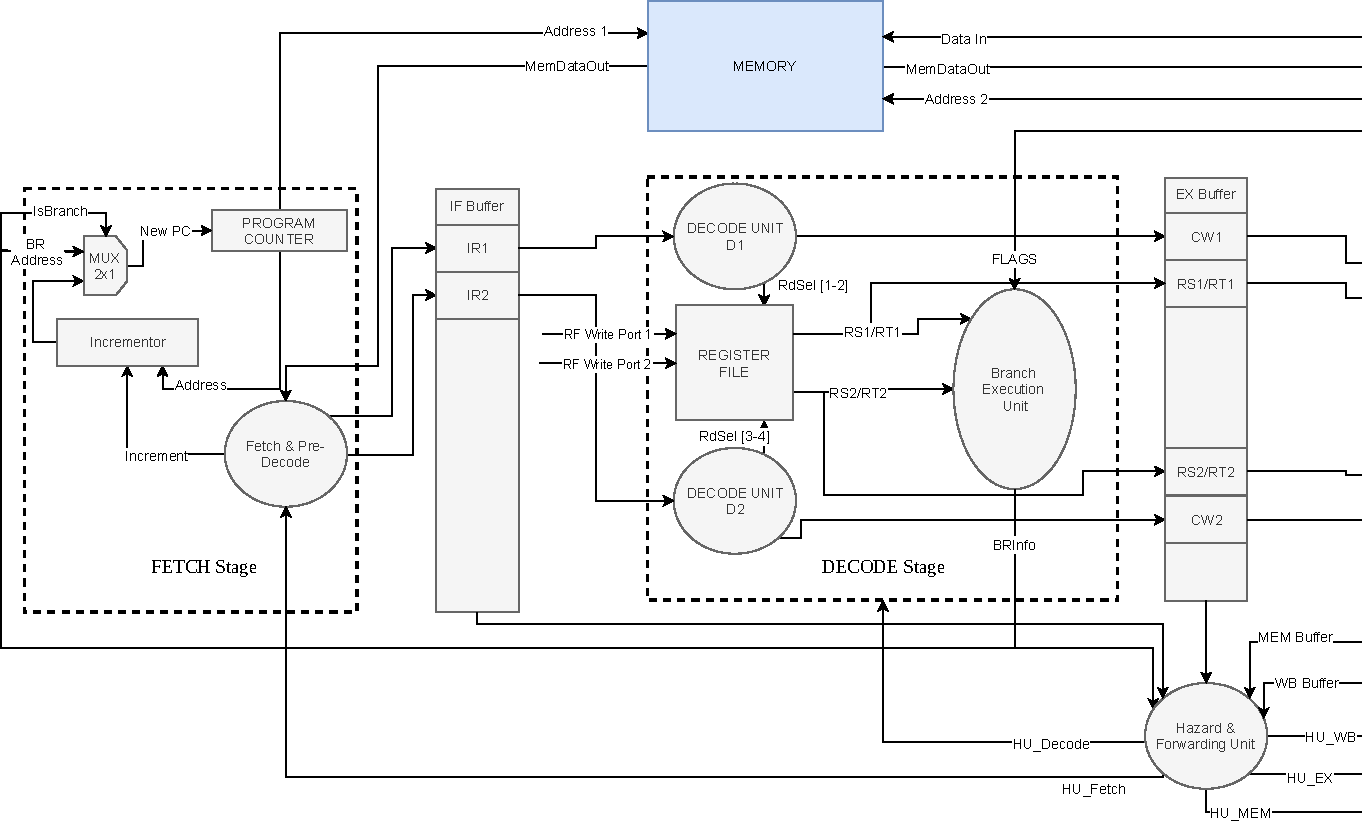
\includegraphics[page=1]{Diagrams/SystemOverviewSplit}
        \caption{Overall Schematic Part 1}
        \label{sys-schematic-1}
    \end{sidewaysfigure}
    \begin{sidewaysfigure}[h]
        \centering
        \includegraphics[page=2]{Diagrams/SystemOverviewSplit}
        \caption{Overall Schematic Part 2}
        \label{sys-schematic-2}
    \end{sidewaysfigure}

\subsection{Memory Unit}
The memory block used is interfaced by two address lines, with the second line given priority whenever a read / write is requested by it. A single word is read or written when an address is on Address2. When an address is on the first line, \textbf{two words} are read at a time starting from the word at the address given by Address1. The first line is only for reading from the memory and has no write option. The read operation is instantaneous while the write operation takes 1 clock cycle (the value is written onto the memory on the falling edge of the clock). 

\subsection{Fetch Stage}
In the fetch stage, the Program Counter (PC) register is connected to Address1 of the memory, the data (from MemDataOut) is then read into the fetch and pre-decode unit which has three outputs: the IRs (Instruction Registers) corresponding to the two streams in Orthrus, IR1 and IR2, as well as the increment to add to the PC for fetching the next instruction. \\
The pre-decode unit handles several issues:
\begin{enumerate}
    \item If an Interrupt or Reset have been latched (we assume that dedicated hardware has already latched them) then the PC is fetched from dedicated memory locations (M[0] for RST and M[1] for ITR) and the appropriate instructions are passed into the pipes.
    \item The unit must do not let two memory-accessing instructions simultaneously into the two streams (since this would result in a structural hazard) and hence passes a No-Op into the second stream when this is detected.
    \item The unit also passes a No-Op into the second stream when an immediate instruction is loaded, since an immediate instruction takes two words.
    \item The unit also passes a No-Op when the two instructions try to use the output port. 
    \item If a CALL or CALL-like instruction is detected, then the next instruction passed is a No-Op (since it will be flushed anyway).
\end{enumerate}
The flow chart for the unit's operation is given by Figure~\ref{fetch-pre-decode-unit}. For the flow chart, the instructions that access memory are: PUSH / POP / LDD / STD / CALL / RET / RTI. In addition to the Pre-Decode unit mentioned, the fetch stage also includes an incrementor to increment the PC as well as a small unit (shown in Figure~\ref{fetch-predecode-npc}) to choose whether to get the PC from the incremented PC, normal branches, from RET / RTI (which are executed in the last stage by necessity of fetching from memory), or from special memory places (for RST / ITR).

\begin{figure}
    \centering
    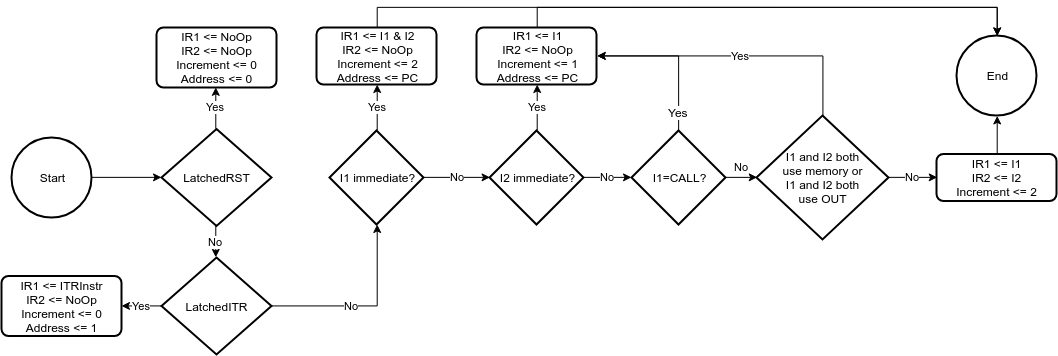
\includegraphics[width=\textwidth]{Diagrams/fetch_predecode_su}
    \caption{Fetch and Pre-Decode Unit Operation}
    \label{fetch-pre-decode-unit}
\end{figure}

\begin{figure}
    \centering
    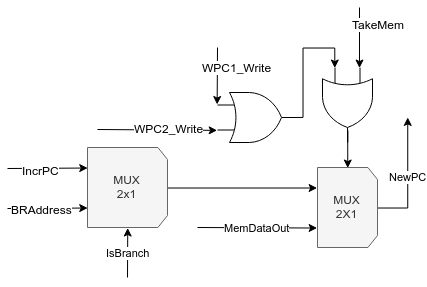
\includegraphics[]{Diagrams/fetch_predecode_npc.png}
    \caption{Next PC MUXing Unit}
    \label{fetch-predecode-npc}
\end{figure}

\subsection{Decode Stage}
The Decode Stage is responsible for translating the received IR into signals that will drive the next stages. Those signals are grouped into a control word, shown in Figure~\ref{control-word}. 
\\ The flow charts in Figures~\ref{decode-chart1} and \ref{decode-chart2} show the decision making process that sets the Control Word.And it is divided into Four branches. 
\begin{enumerate}
\item One-Operand Instructions: At which the decode stage passes the ALU Operation, the contents and address of the destination register (RT) and since they are one-operand instructions, the source register (RS) is nonexistent and thus its value is passed as 0 to the ALU.
\item Two-Operand Instructions: If the instruction is of type shift, the Decoding unit extends the shift amount (Shamt in IR) and places into RT and forwards value of RS register for ALU operation. As for other instructions, RT and RS values and addresses are both forwarded. 
\item Memory Operation: If Push or Pop, it sets the ALU op to F= SP-1 and F= SP+1 respectively (the ALU has a dedicated incrementor-decrementor for the SP register, as it is 32b vs all other outputs being 16b). As for Loads and Stores, needed values are just passed along. (F=B)
\item Branching: Branching check is done in the decoding stage, and if condition is true, RT value is input to PC. By setting IsBranch and Branch Address. 
\end{enumerate}
\begin{figure}
    \centering
    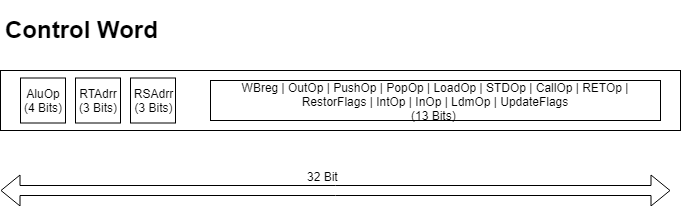
\includegraphics[width=\textwidth,height=\textheight,keepaspectratio]{Diagrams/ControlWord.png}
    \caption{Control Word}
    \label{control-word}
\end{figure}

\begin{figure}
    \centering
    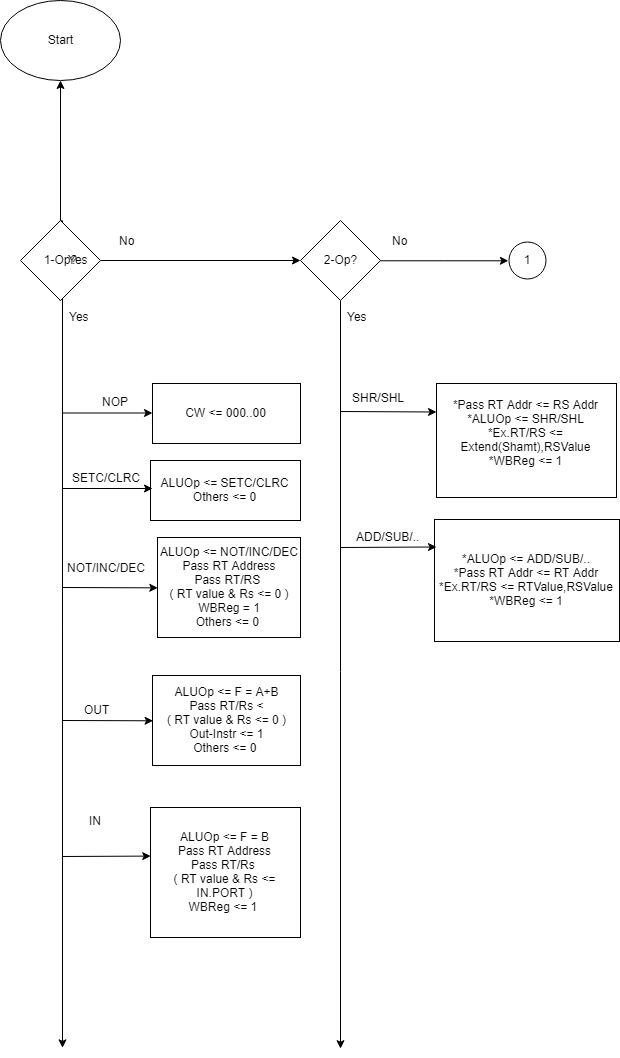
\includegraphics[height=0.9\textheight,keepaspectratio]{Diagrams/decode_1.png}
    \caption{Decode Flow Chart P1}
    \label{decode-chart1}
\end{figure}

\begin{figure}
    \centering
    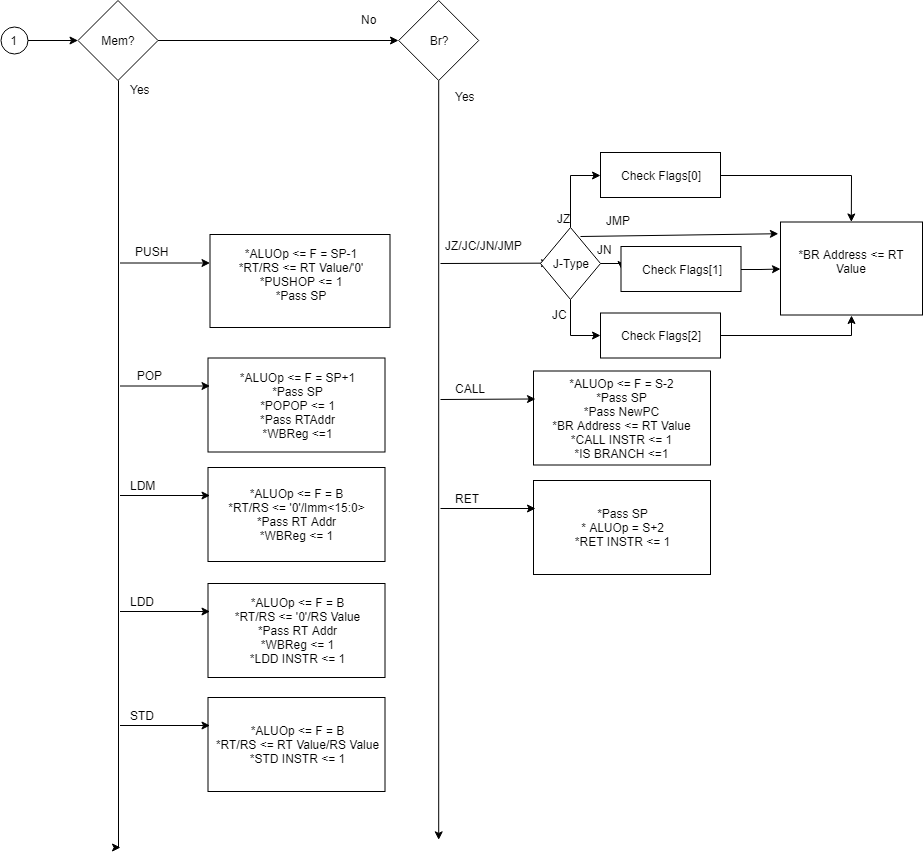
\includegraphics[width=\textwidth,height=\textheight,keepaspectratio]{Diagrams/decode_2.png}
    \caption{Decode Flow Chart P2}
    \label{decode-chart2}
\end{figure}

\subsection{Execute Stage}
In execute stage, set logic is carried out by ALU and the Flag register is set accordingly. The two Pipes edit ONE flag register, and due to its latency in sequence, pipe 2 is prioritized when a conflict arises in setting the flags. It is a simple issue to handle as show in Figure~\ref{flag-reg}, there was no need for the Hazard unit to handle it. In addition to the shown logic, a few simple MUXs (not shown) are responsible for copying the FLAGs register into the FLAGS\textunderscore{LNK} register (or restoring it) when INTR/RTI are detected, respectively.
\begin{figure}
    \centering
    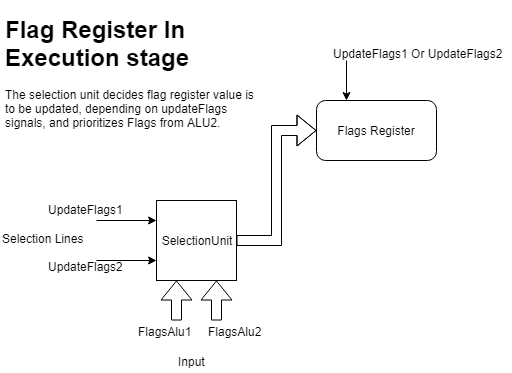
\includegraphics[width=\textwidth,keepaspectratio]{Diagrams/FlagRegister.png}
    \caption{Flag Register}
    \label{flag-reg}
\end{figure}

\subsection{Memory Stage}
In the Memory access stage, according to operation type, MAddr (The address to send the memory) and MData (The data to send the memory / also receives the data in Store operations) are set if needed (load for example doesn't need MData to be set) as shown in the flow chart in Figure~\ref{memory-chart}. In addition to managing this, the memory stage unit also outputs signal WPC\textunderscore{Write} when the PC's value should be taken from the memory.
\begin{figure}
    \centering
    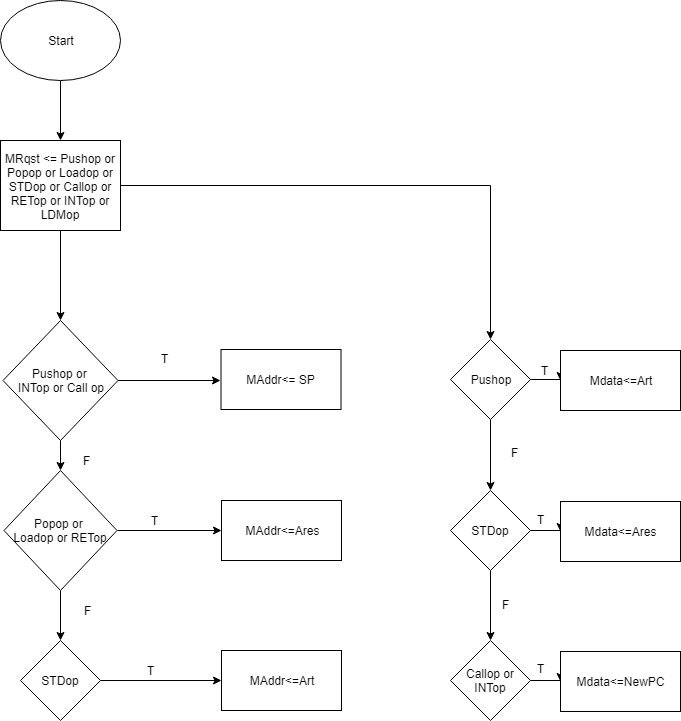
\includegraphics[width=\textwidth,height=\textheight,keepaspectratio]{Diagrams/MemoryStage.png}
    \caption{Memory Stage}
    \label{memory-chart}
\end{figure}

\subsection{Write Back Stage}
In the write back stage, we have to deal with the following outcomes
 \begin{enumerate}
\item Writing back to the R[RT] the Value in ARes if the current operation involves writing to a register.
\item Writing to the Out port the value in ARes.
\item Updating SP values with ARes if it was any operation that changes the SP.
\item Nothing needs to be written back, the stage does nothing.
\end{enumerate}

\begin{figure}
    \centering
    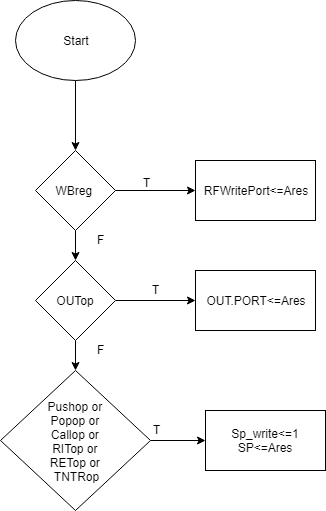
\includegraphics[]{Diagrams/WBStage.png}
    \caption{Write Back Stage}
    \label{WB-chart}
\end{figure}

\subsection{Hazard Detection Unit}
For clarity, the hazard detection wires aren't wired in the overall schematic into the components inside each stage. To be as clear as possible, we mention our assumptions:
\begin{enumerate}
    \item A \textbf{stall} input is available to all components. When this input is set to true, the component passes zeros (i.e. a No-Op) as an output regardless of the input present in the previous buffer.
    \item A \textbf{flush} input is available to all pipeline register buffers, when turned on the by the detection unit all the pipeline buffers are immediately replaced by zeros. This helps us correct mispredicted branches.
    \item If some line is forwarded by the Hazard unit to any stage, it \textbf{MUST} be taken by that stage instead of the original line. So if, for example, a line is shown in the schematic as connected to the RS line coming in from the register buffer but the Hazard unit forwards another input then the new input must be taken instead. Every forwarded line has an associated bit that tells the stage whether or not to take it.
\end{enumerate}
We deal with three types of Hazards:
\begin{enumerate}
\item The only data hazards that affect the system are RAW data hazards, as the system's sequential integrity is preserved by making sure stalls affect both pipes. WAR hazards have no impact because we send the needed data into the separate pipeline registers when needed, RAR hazards cause no problems, and WAW hazards on different registers do not affect the system's correctness because they write in separate places. Since pipe 2 (the lower pipe) has the later instruction in sequence extra precautions for data dependencies were taken as shown in the figures. Figure~\ref{raw-chart} shows how RAW hazards (to the general purpose registers) are handled and Figure~\ref{raw1-chart} shows the checks made when handling the SP, since it is on its own accord in the pipe. A Special case is in branch operations for RT that should contain memory address to branch address as shown in figure~\ref{RAW-BR}.
\item Structural Hazards: WAW hazards on the same register are handled by enforcing a priority system with the higher priority of writing to some register given to the second pipe since it is the one containing the newer instruction, as shown in Figure~\ref{wbwb-chart}.
\\ Because this is a Von-Neumann architecture, we have only one memory: A structural hazard arises when fetching instructions while simultaneously accessing the memory (since the memory can only be read from one address at a time), in this case the MEM stage is given priority by stalling the fetch. See Figure~\ref{mem-chart}. A similar hazard arises if both pipes desire access for the memory, this is solved by not allowing two memory-accessing instructions together back in the Fetch Stage.
\item Control Hazards: The following are the main hazards:
\begin{enumerate}
    \item We always predict not taken in branches. If the prediction fails, then the fetch instruction preceding it is flushed. 
    \item If a CALL or unconditional JMP is detected, then the instructions in Fetch are flushed. If RET or RTI are detected, then no new instructions are loaded until the new PC value is fetched (in the memory stage), as shown in Figure~\ref{control}.
    \item If either an INT signal or a RST signal is detected, no new instructions are fetched, then the Fetch Stage handles this by changing the PC to the appropriate value directly, and there is no need for the hazard to be handled elsewhere.
\end{enumerate}
\end{enumerate}

\begin{figure}
    \centering
    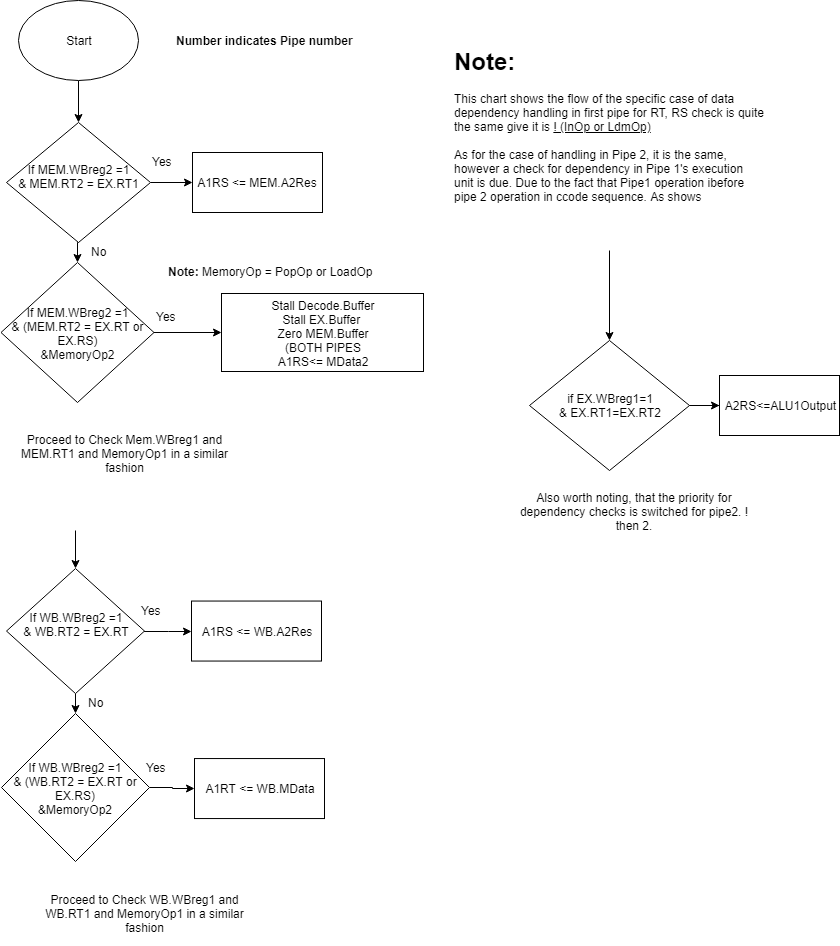
\includegraphics[width=\textwidth,height=\textheight,keepaspectratio]{Diagrams/RawDataDependency1.png}
    \caption{RAW Data Hazards - General}
    \label{raw-chart}
\end{figure}

\begin{figure}
    \centering
    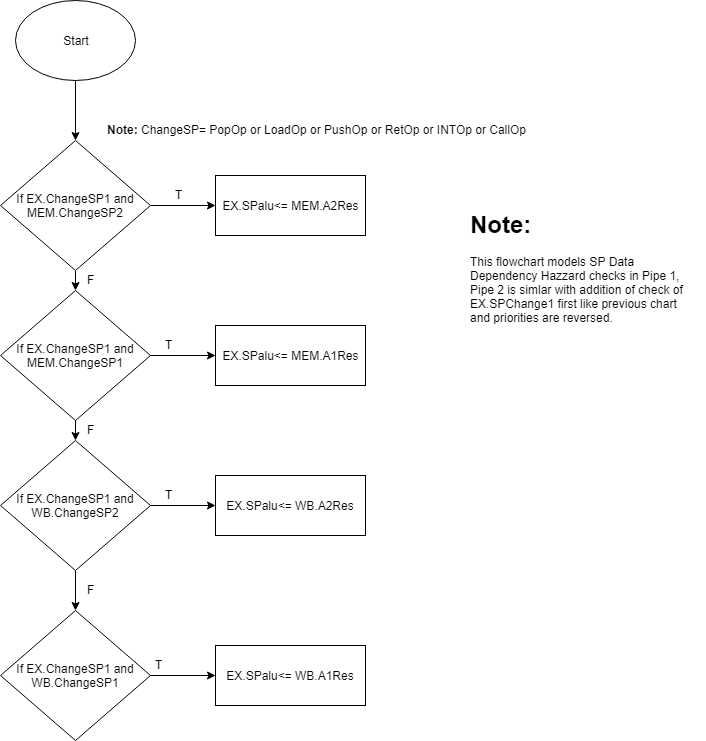
\includegraphics[width=\textwidth,keepaspectratio]{Diagrams/RawDataDependency2.png}
    \caption{RAW Data Hazards - SP}
    \label{raw1-chart}
\end{figure}


\begin{figure}
    \centering
    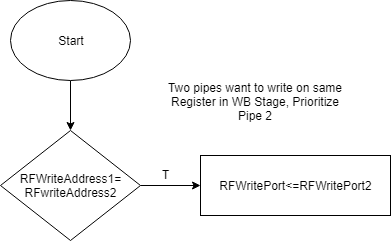
\includegraphics[width=0.4\textheight]{Diagrams/WawDataDependency_Structural.png}
    \caption{WB-WB Hazard}
    \label{wbwb-chart}
\end{figure}

\begin{figure}
    \centering
    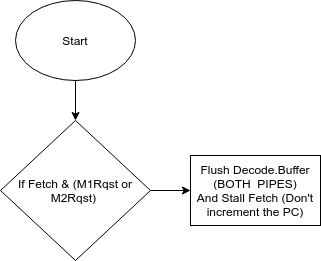
\includegraphics[height=0.3\textheight,keepaspectratio]{Diagrams/FetchMem.png}
    \caption{Fetch-MEM and MEM-MEM Hazards}
    \label{mem-chart}
\end{figure}


\begin{figure}
    \centering
    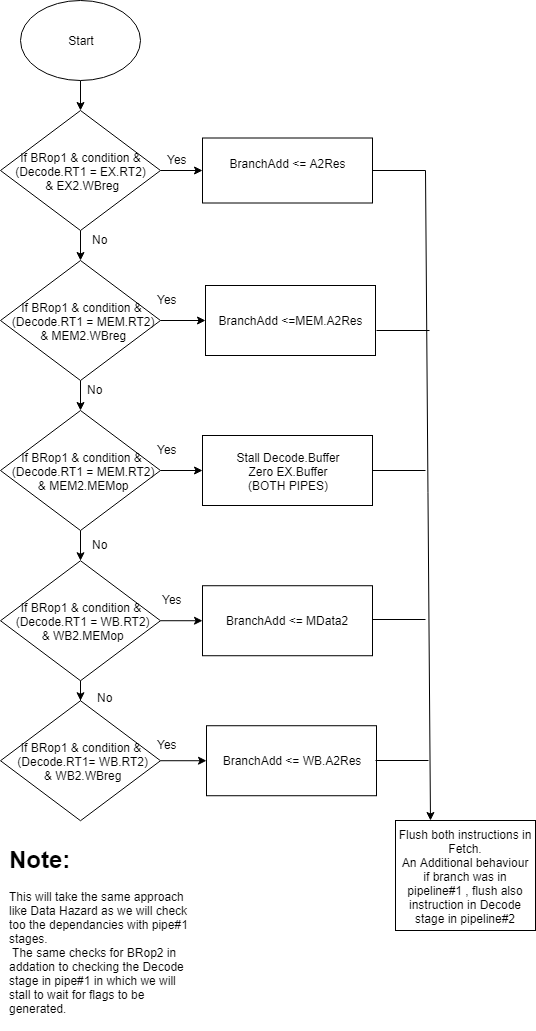
\includegraphics[height=0.9\textheight,keepaspectratio]{Diagrams/Hazard.png}
    \caption{RAW for RT in Branch Instruction}
    \label{RAW-BR}
\end{figure}


\begin{figure}
    \centering
    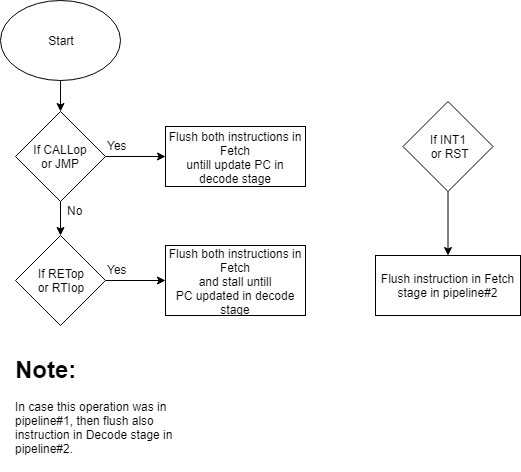
\includegraphics[width=\textwidth,keepaspectratio]{Diagrams/ControlHazard1.png}
    \caption{Control Hazard - CALL/JMP/RET/RTI}
    \label{control}
\end{figure}

% --------------------------------------------------------------
%     You don't have to mess with anything below this line.
% --------------------------------------------------------------
			
\end{document}	